\documentclass[shortpres,usenames,dvipsnames]{beamer}
\usetheme{CambridgeUS}

% Depending on build configuration, one of these packages will
% enable unicode
\usepackage[utf8]{inputenc}
\usepackage{fontspec}
\usepackage{listings}

%Images
\usepackage{graphicx, svg}
\usepackage{caption}
\usepackage{adjustbox}

%Mixed
\usepackage{subfig}
\usepackage{multicol}
\usepackage{color}
\usepackage{pgfplots}
\usepackage{xmpmulti}
\usepackage{verbatim}

%Tikz
\usepackage{tikz}
\usepackage{environ}
\usetikzlibrary{positioning}



\usepackage{algorithm,algpseudocode}  %for algorithm environmenstacle in the bathymetry to show the effect of the soruce terms in 2D.t

\setbeamertemplate{footline}
{
	\leavevmode%
	\hbox{%
		\begin{beamercolorbox}[wd=.333333\paperwidth,ht=2.25ex,dp=1ex,center]{author in head/foot}%
			\usebeamerfont{author in head/foot}\insertshortauthor%~~\beamer@ifempty{\insertshortinstitute}{}{(\insertshortinstitute)}
		\end{beamercolorbox}%
		\begin{beamercolorbox}[wd=.333333\paperwidth,ht=2.25ex,dp=1ex,center]{title in head/foot}%
			\usebeamerfont{title in head/foot}\insertshorttitle
		\end{beamercolorbox}%
		\begin{beamercolorbox}[wd=.333333\paperwidth,ht=2.25ex,dp=1ex,right]{date in head/foot}%
			\usebeamerfont{date in head/foot}\insertshortdate{}\hspace*{2em}
			\insertframenumber{} / \inserttotalframenumber\hspace*{2ex}
		\end{beamercolorbox}}%
		\vskip0pt%
	}\part{title}
	\beamertemplatenavigationsymbolsempty
	
	
	%color specification---------------------------------------------------------------
	\definecolor{TUMblue}{rgb}{0.00, 0.40, 0.74}
	\definecolor{TUMgray}{rgb}{0.85, 0.85, 0.86}
	\definecolor{TUMpantone285C}{rgb}{0.00, 0.45, 0.81}
	\definecolor{lightblue}{rgb}{0.7529,0.8118,0.9333}
	
	\setbeamercolor{block title}{fg=white, bg=TUMpantone285C}
	\setbeamercolor{block body}{bg=lightblue}
	\setbeamertemplate{blocks}[rounded][shadow=true]
	%----------------------------------------------------------------------------------
	
	\setbeamercolor{frametitle}{fg=TUMblue, bg=white}
	\setbeamercolor{palette primary}{fg=TUMblue,bg=TUMgray}
	\setbeamercolor{palette secondary}{use=palette primary,fg=TUMblue,bg=white}
	\setbeamercolor{palette tertiary}{use=palette primary,fg=white, bg=TUMblue}
	\setbeamercolor{palette quaternary}{use=palette primary,fg=white,bg=TUMpantone285C}
	
	
	\setbeamercolor{title}{bg=white,fg=TUMblue}
	\setbeamercolor{item projected}{use=item,fg=black,bg = lightblue}
	\setbeamercolor{block title}{fg=black, bg=lightblue}
	\setbeamercolor{block body}{bg=white}
	\setbeamertemplate{blocks}[rounded][shadow=true]
	%----------------------------------------------------------------------------------
	
	
	%############### Self defined commands ##############################
	\newcommand{\imgvoffset}{-20pt}
	\newcommand{\texthoffset}{20pt}
	\newcommand{\imgfullscale}{0.75}
	\newcommand{\imgcolscale}{0.9}
	
	\captionsetup[subfigure]{labelformat=empty}		%Disable enumeration of subfigures
	%####################################################################
	
	%############### Title information ###############
	\title[{Tsunami simulation}]{Assignment 4}
	\author[Bellamy, Honal, Wieser]{Gruppe 03\\George Bellamy, Christoph Honal, Felix Wieser\\\vspace{10pt}{\small Bachelorpraktikum}}
	\institute[TU M\"unchen]{Technical University of Munich}
	\date{9. Januar 2018}
	%#################################################
	
	%############### Tikz picture configuration ###############
	\newcommand{\pgfglobalscale}{0.7}
	\newcommand{\pgfglobalheadervspace}{\vspace{5pt}\\}
	%##########################################################
	
	\lstset{escapeinside={<@}{@>}}
	
	\begin{document}
		\maketitle
		
\begin{frame}{Overview}
	\begin{figure}
		\subfloat[HPC]{\includegraphics[clip,width=0.3\linewidth]
			{img/lrz.png}}
		\hspace{20pt}
		\subfloat[Coarse computation]{
\includegraphics[clip,width=0.3\linewidth]
			{img/tuhoku_mixed.png}}
		\hspace{40pt}\vspace{10pt}\\
		\subfloat[Project*]{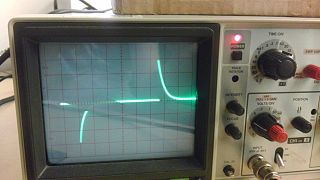
\includegraphics[clip,width=0.3\linewidth]
			{img/oszi.jpg}}
		\vfill
		\flushleft
		{\fontsize{5}{5} \selectfont *Image: https://commons.wikimedia.org/wiki/File:1tt.jpg}
	\end{figure}
\end{frame}

\begin{frame}[fragile]{HPC: Performance analysis (Overview)}
	\textbf{Analysis overview}
	\begin{itemize}
		\item HPC $\leftrightarrow$ PC
		\item \verb|GCC| $\leftrightarrow$ Intel
		\item OpenMP: Basic \verb|for| parallelisation
		\item OpenMP: \verb|assert|, thread workload optimisation, math, \dots
	\end{itemize}
	
	\vspace{10pt}
	\textbf{Performance profiles}\\
	\begin{tabular}{lllll}
		name & scenario & cells & comp. time [s] & checkpoints\\
		\hline
		light & Tuhoku & 500² & 1000 & 300\\
		heavy & Tuhoku & 5000² & 30000 & 1000\\
	\end{tabular}
\end{frame}

\begin{frame}{HPC: Performance analysis (HPC $\leftrightarrow$ PC)}
	\centering
	\begin{tikzpicture}
		\node[](h){\textbf{Wall clock time analysis}};
		\node[below=5pt of h.south](A){
			\begin{tikzpicture}[scale=\pgfglobalscale]
			\begin{axis}[
			xbar, xmin=0, xmax=15,
			width=13cm, height=3.5cm, enlarge y limits=0.6,
			xlabel={wall clock time [s]},
			xlabel style={at={(axis description cs:0.5,-0.25)}, anchor=south},
			x tick label style={rotate=0},
			xtick distance=5,
			symbolic y coords={light},
			ytick=data,
			%ylabel=Profile,
			ylabel style={at={(axis description cs:-0.05,0.2)},anchor=west},
			nodes near coords, nodes near coords align={horizontal},
			legend pos=south east,
			]
			\addplot coordinates {(9,light)};	%28 threads
			\addplot coordinates {(7,light)};	%28 threads
			\addplot coordinates {(7,light)};	%56 threads
			\legend{PC (28 threads),HPC (28 threads),HPC (56 threads)}
			\end{axis}
			\end{tikzpicture}
		};
		\node[below=10pt of A.south](B){
			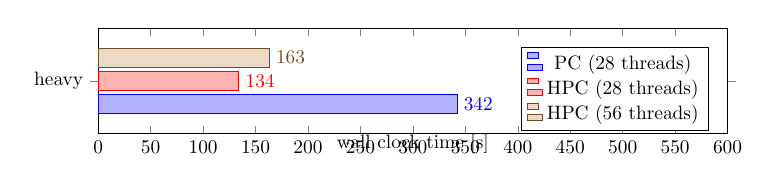
\begin{tikzpicture}[scale=\pgfglobalscale]
			\begin{axis}[
			xbar, xmin=0, xmax=600,
			width=13cm, height=3.5cm, enlarge y limits=0.6,
			xlabel={wall clock time [s]},
			xlabel style={at={(axis description cs:0.5,-0.25)}, anchor=south},
			x tick label style={rotate=0},
			xtick distance=50,
			symbolic y coords={light,heavy},
			ytick=data,
			%ylabel=Profile,
			ylabel style={at={(axis description cs:-0.05,0.2)},anchor=west},
			nodes near coords, nodes near coords align={horizontal},
			legend pos=south east,
			]
			\addplot coordinates {(342,heavy)};	%28 threads
			\addplot coordinates {(134,heavy)};	%28 threads
			\addplot coordinates {(163,heavy)};	%56 threads
			\legend{PC (28 threads),HPC (28 threads),HPC (56 threads)}
			\end{axis}
			\end{tikzpicture}
		};
	\end{tikzpicture}
	\newline
	{\tiny GNU, all optimizations, release}
\end{frame}

\begin{frame}{HPC: Performance analysis (HPC $\leftrightarrow$ PC)}
	\centering
	\begin{tikzpicture}
		\node[](h){\textbf{Computation time analysis}};
		\node[below=5pt of h.south](A){
			\begin{tikzpicture}[scale=\pgfglobalscale]
			\begin{axis}[
			xbar, xmin=0, xmax=30,
			width=13cm, height=3.5cm, enlarge y limits=0.6,
			xlabel={cpu time [s]},
			xlabel style={at={(axis description cs:0.5,-0.25)}, anchor=south},
			x tick label style={rotate=0},
			xtick distance=5,
			symbolic y coords={light},
			ytick=data,
			%ylabel=Profile,
			ylabel style={at={(axis description cs:-0.05,0.2)},anchor=west},
			nodes near coords, nodes near coords align={horizontal},
			legend pos=south east,
			]
			\addplot coordinates {(5.38,light)};	%28 threads
			\addplot coordinates {(14.2,light)};	%28 threads
			\addplot coordinates {(4.3,light)};		%56 threads
			\legend{PC (28 threads),HPC (28 threads),HPC (56 threads)}
			\end{axis}
			\end{tikzpicture}
		};
		\node[below=10pt of A.south](B){
			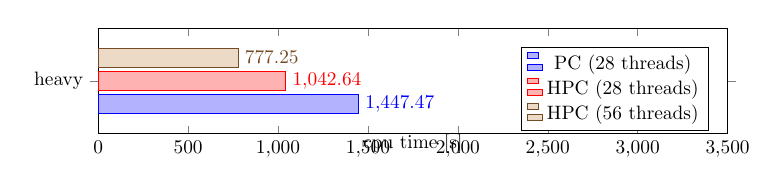
\begin{tikzpicture}[scale=\pgfglobalscale]
			\begin{axis}[
			xbar, xmin=0, xmax=3500,
			width=13cm, height=3.5cm, enlarge y limits=0.6,
			xlabel={cpu time [s]},
			xlabel style={at={(axis description cs:0.5,-0.25)}, anchor=south},
			x tick label style={rotate=0},
			xtick distance=500,
			symbolic y coords={light,heavy},
			ytick=data,
			%ylabel=Profile,
			ylabel style={at={(axis description cs:-0.05,0.2)},anchor=west},
			nodes near coords, nodes near coords align={horizontal},
			legend pos=south east,
			]
			\addplot coordinates {(1447.47,heavy)};	%28 threads
			\addplot coordinates {(1042.64,heavy)};	%28 threads
			\addplot coordinates {(777.25,heavy)};	%56 threads
			\legend{PC (28 threads),HPC (28 threads),HPC (56 threads)}
			\end{axis}
			\end{tikzpicture}
		};
	\end{tikzpicture}
	\newline
	{\tiny GNU, all optimizations, release}
\end{frame}

\begin{frame}{HPC: Performance analysis (HPC $\leftrightarrow$ PC)}
	\centering
	\textbf{Analysis}
	\begin{itemize}
		\item Huge impact of context switching on execution time
		\item Computed data of HPC and PC are identical
	\end{itemize}
	%TODO: Implement content
\end{frame}

\begin{frame}{HPC: Performance analysis (GCC $\leftrightarrow$ Intel)}
	\centering
	\begin{tikzpicture}
		\node[](h){\textbf{Wall clock time analysis}};
		\node[below=5pt of h.south](A){
			\begin{tikzpicture}[scale=\pgfglobalscale]
			\begin{axis}[
			xbar, xmin=0, xmax=12,
			width=13cm, height=4cm, enlarge y limits=0.6,
			xlabel={wall clock time [s]},
			x label style={at={(axis description cs:0.5,-0.22)}, anchor=south},
			x tick label style={rotate=-45},
			symbolic y coords={light},
			ytick=data,
			%ylabel=Profile,
			y label style={at={(axis description cs:-0.05,0.2)},anchor=west},
			x tick label style={rotate=45},
			xtick distance=2,
			nodes near coords, nodes near coords align={horizontal},
			legend pos=south east,
			]
			\addplot coordinates {(7,light)};	%Gnu, 28 threads
			\addplot coordinates {(7,light)};	%Intel, 28 threads
			\addplot coordinates {(7,light)};	%Gnu, 56 threads
			\addplot coordinates {(6,light)};	%Intel, 56 threads
			\legend{gnu (28 threads),intel (28 threads),gnu (56 threads),intel (56 threads)}
			\end{axis}
			\end{tikzpicture}
		};
		\node[below=10pt of A.south](B){
			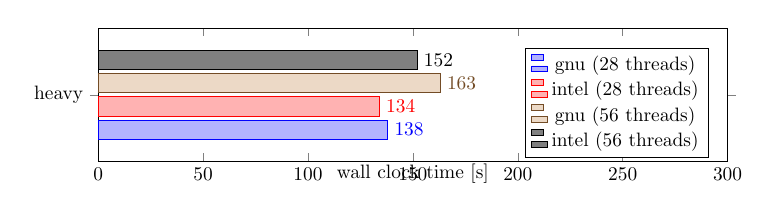
\begin{tikzpicture}[scale=\pgfglobalscale]
			\begin{axis}[
			xbar, xmin=0, xmax=300,
			width=13cm, height=4cm, enlarge y limits=0.6,
			xlabel={wall clock time [s]},
			x label style={at={(axis description cs:0.5,-0.22)}, anchor=south},
			x tick label style={rotate=-45},
			symbolic y coords={heavy},
			ytick=data,
			%ylabel=Profile,
			y label style={at={(axis description cs:-0.05,0.2)},anchor=west},
			x tick label style={rotate=45},
			xtick distance=50,
			nodes near coords, nodes near coords align={horizontal},
			legend pos=south east,
			]
			\addplot coordinates {(138,heavy)};	%Gnu, 28 threads
			\addplot coordinates {(134,heavy)};	%Intel, 28 threads
			\addplot coordinates {(163,heavy)};	%Gnu, 56 threads
			\addplot coordinates {(152,heavy)};	%Intel, 56 threads
			\legend{gnu (28 threads),intel (28 threads),gnu (56 threads),intel (56 threads)}
			\end{axis}
			\end{tikzpicture}
		};
	\end{tikzpicture}
	\newline
	{\tiny All optimisations, release}
\end{frame}

\begin{frame}{HPC: Performance analysis (GCC $\leftrightarrow$ Intel)}
	\centering
	\begin{tikzpicture}
		\node[](h){\textbf{Computation time analysis}};
		\node[below=5pt of h.south](A){
			\begin{tikzpicture}[scale=\pgfglobalscale]
			\begin{axis}[
			xbar, xmin=0, xmax=28,
			width=13cm, height=4cm, enlarge y limits=0.6,
			xlabel={cpu time [s]},
			x label style={at={(axis description cs:0.5,-0.22)}, anchor=south},
			x tick label style={rotate=-45},
			symbolic y coords={light},
			ytick=data,
			%ylabel=Profile,
			y label style={at={(axis description cs:-0.05,0.2)},anchor=west},
			x tick label style={rotate=45},
			xtick distance=5,
			nodes near coords, nodes near coords align={horizontal},
			legend pos=south east,
			]
			\addplot coordinates {(13.04,light)};	%Gnu, 28 threads
			\addplot coordinates {(9.55,light)};	%Intel, 28 threads
			\addplot coordinates {(4.3,light)};	%Gnu, 56 threads
			\addplot coordinates {(5.45,light)};	%Intel, 56 threads
			\legend{gnu (28 threads),intel (28 threads),gnu (56 threads),intel (56 threads)}
			\end{axis}
			\end{tikzpicture}
		};
		\node[below=10pt of A.south](B){
			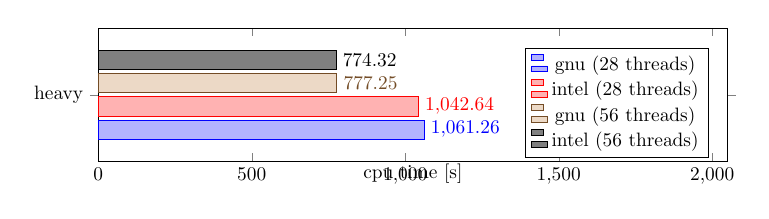
\begin{tikzpicture}[scale=\pgfglobalscale]
			\begin{axis}[
			xbar, xmin=0, xmax=2050,
			width=13cm, height=4cm, enlarge y limits=0.6,
			xlabel={cpu time [s]},
			x label style={at={(axis description cs:0.5,-0.22)}, anchor=south},
			x tick label style={rotate=-45},
			symbolic y coords={heavy},
			ytick=data,
			%ylabel=Profile,
			y label style={at={(axis description cs:-0.05,0.2)},anchor=west},
			x tick label style={rotate=45},
			xtick distance=500,
			nodes near coords, nodes near coords align={horizontal},
			legend pos=south east,
			]
			\addplot coordinates {(1061.26,heavy)};	%Gnu, 28 threads
			\addplot coordinates {(1042.64,heavy)};	%Intel, 28 threads
			\addplot coordinates {(777.25,heavy)};	%Gnu, 56 threads
			\addplot coordinates {(774.32,heavy)};	%Intel, 56 threads
			\legend{gnu (28 threads),intel (28 threads),gnu (56 threads),intel (56 threads)}
			\end{axis}
			\end{tikzpicture}
		};
	\end{tikzpicture}
	\newline
	{\tiny All optimisations, release}
\end{frame}

\begin{frame}{HPC: Performance analysis (GCC $\leftrightarrow$ Intel)}
	\textbf{Analysis}
	\begin{itemize}
		\item
		\item 
		\item
		%TODO: Implement content
	\end{itemize}
\end{frame}

\begin{frame}[containsverbatim]{OpenMP: Basic for parallelisation}
	\begin{multicols}{2}
		\textbf{Inner loop parallelisation}
		\begin{lstlisting}[
		language=C++,
		basicstyle=\tiny, numbers=left, stepnumber=1, keywordstyle=\color{blue}\ttfamily,
		stringstyle=\color{red}\ttfamily,
		commentstyle=\color{ForestGreen}\ttfamily,
		xleftmargin=.04\textwidth, xrightmargin=.2\textwidth,
		tabsize=3,
		gobble=6,
		]
		for(int y = 0; y < numRows(); y++)
		{
			//Parallelisation of inner loop
			<@\texttt{\textcolor{orange}{\#pragma parallel for}}@>
			for(int x = 0; x < numCols(); x++)
			{
				doSomething(x,y);
			}
		}
		\end{lstlisting}
		
		\begin{itemize}
			\item Each thread processes one \verb|doSomething()|
			\item Many context switches
			\item Short thread lifetime
			\item[$\Rightarrow$] Bad performance 
		\end{itemize}
		
		\columnbreak
		
		\textbf{Outer loop parallelisation}
		\begin{lstlisting}[
		language=C++,
		basicstyle=\tiny, numbers=left, stepnumber=1, keywordstyle=\color{blue}\ttfamily,
		stringstyle=\color{red}\ttfamily,
		commentstyle=\color{ForestGreen}\ttfamily,
		xleftmargin=.04\textwidth, xrightmargin=.2\textwidth,
		tabsize=3,
		gobble=6,
		]
		//Parallelisation of outer loop
		<@\texttt{\textcolor{orange}{\#pragma parallel for}}@>
		for(int y = 0; y < numRows(); y++)
		{
			for(int x = 0; x < numCols(); x++)
			{
				doSomething(x,y);
			}
		}
		\end{lstlisting}
		
		\begin{itemize}
			\item Each thread executes one row
			\item Less context switches
			\item Increased thread lifetime
			\item[$\Rightarrow$] Better performance
		\end{itemize}
	\end{multicols}
\end{frame}

\begin{frame}[fragile]{OpenMP: Advanced parallelisation}
	\textbf{Custom thread scheduling}
	\begin{itemize}
		\item TODO
	\end{itemize}
	%TODO: Enhance content
	
	\vspace{20pt}
	
	\textbf{Further improvements}
	\begin{itemize}
		\item Toggle for \verb|assert| statements
	\end{itemize}
\end{frame}

\begin{frame}{OpenMP: Advanced parallelisation}
	\centering
	\begin{tikzpicture}
		\node[](h){\textbf{Wall clock time analysis}};
		\node[below=5pt of h.south](A){
			\begin{tikzpicture}[scale=\pgfglobalscale]
			\begin{axis}[
			xbar, xmin=0, xmax=15,
			width=13cm, height=4cm, enlarge y limits=0.6,
			xlabel={wall clock time [s]},
			x label style={at={(axis description cs:0.5,-0.22)}, anchor=south},
			x tick label style={rotate=-45},
			symbolic y coords={light},
			ytick=data,
			%ylabel=Profile,
			y label style={at={(axis description cs:-0.05,0.2)},anchor=west},
			x tick label style={rotate=45},
			xtick distance=5,
			nodes near coords, nodes near coords align={horizontal},
			legend pos=south east,
			]
			\addplot coordinates {(7,light)};	%Original, 28 threads
			\addplot coordinates {(7,light)};	%Optimized, 28 threads
			\addplot coordinates {(7,light)};		%Original, 56 threads
			\addplot coordinates {(7,light)};	%Optimized, 56 threads
			\legend{original (28 threads),optimized (28 threads),original (56 threads),optimized (56 threads)}
			\end{axis}
			\end{tikzpicture}
		};
		\node[below=10pt of A.south](B){
			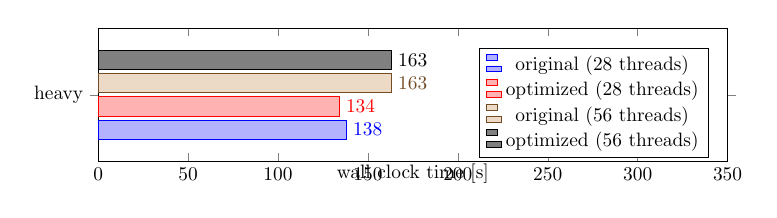
\begin{tikzpicture}[scale=\pgfglobalscale]
			\begin{axis}[
			xbar, xmin=0, xmax=350,
			width=13cm, height=4cm, enlarge y limits=0.6,
			xlabel={wall clock time [s]},
			x label style={at={(axis description cs:0.5,-0.22)}, anchor=south},
			x tick label style={rotate=-45},
			symbolic y coords={heavy},
			ytick=data,
			%ylabel=Profile,
			y label style={at={(axis description cs:-0.05,0.2)},anchor=west},
			x tick label style={rotate=45},
			xtick distance=50,
			nodes near coords, nodes near coords align={horizontal},
			legend pos=south east,
			]
			\addplot coordinates {(138,heavy)};	%Original, 28 threads
			\addplot coordinates {(134,heavy)};	%Optimized, 28 threads
			\addplot coordinates {(163,heavy)};	%Original, 56 threads
			\addplot coordinates {(163,heavy)};	%Optimized, 56 threads
			\legend{original (28 threads),optimized (28 threads),original (56 threads),optimized (56 threads)}
			\end{axis}
			\end{tikzpicture}
		};
	\end{tikzpicture}
	\newline
	{\tiny GNU, release}
\end{frame}

\begin{frame}{OpenMP: Advanced parallelisation}
	\centering
	\begin{tikzpicture}
		\node[](h){\textbf{Computation time analysis}};
		\node[below=5pt of h.south](A){
			\begin{tikzpicture}[scale=\pgfglobalscale]
			\begin{axis}[
			xbar, xmin=0, xmax=28,
			width=13cm, height=4cm, enlarge y limits=0.6,
			xlabel={cpu time [s]},
			x label style={at={(axis description cs:0.5,-0.22)}, anchor=south},
			x tick label style={rotate=-45},
			symbolic y coords={light},
			ytick=data,
			%ylabel=Profile,
			y label style={at={(axis description cs:-0.05,0.2)},anchor=west},
			x tick label style={rotate=45},
			xtick distance=5,
			nodes near coords, nodes near coords align={horizontal},
			legend pos=south east,
			]
			\addplot coordinates {(13.04,light)};	%Original, 28 threads
			\addplot coordinates {(14.20,light)};	%Optimized, 28 threads
			\addplot coordinates {(4.35,light)};		%Original, 56 threads
			\addplot coordinates {(4.30,light)};	%Optimized, 56 threads
			\legend{original (28 threads),optimized (28 threads),original (56 threads),optimized (56 threads)}
			\end{axis}
			\end{tikzpicture}
		};
		\node[below=10pt of A.south](B){
			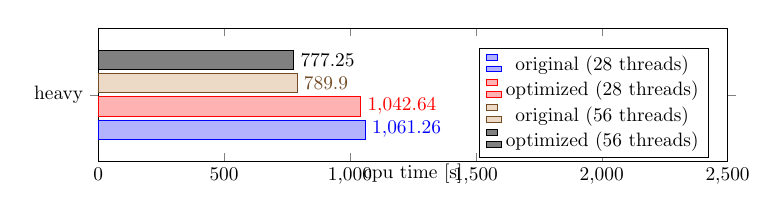
\begin{tikzpicture}[scale=\pgfglobalscale]
			\begin{axis}[
			xbar, xmin=0, xmax=2500,
			width=13cm, height=4cm, enlarge y limits=0.6,
			xlabel={cpu time [s]},
			x label style={at={(axis description cs:0.5,-0.22)}, anchor=south},
			x tick label style={rotate=-45},
			symbolic y coords={heavy},
			ytick=data,
			%ylabel=Profile,
			y label style={at={(axis description cs:-0.05,0.2)},anchor=west},
			x tick label style={rotate=45},
			xtick distance=500,
			nodes near coords, nodes near coords align={horizontal},
			legend pos=south east,
			]
			\addplot coordinates {(1061.26,heavy)};	%Original, 28 threads
			\addplot coordinates {(1042.64,heavy)};	%Optimized, 28 threads
			\addplot coordinates {(789.90,heavy)};	%Original, 56 threads
			\addplot coordinates {(777.25,heavy)};	%Optimized, 56 threads
			\legend{original (28 threads),optimized (28 threads),original (56 threads),optimized (56 threads)}
			\end{axis}
			\end{tikzpicture}
		};
	\end{tikzpicture}
	\newline
	{\tiny GNU, release}
\end{frame}

\begin{frame}{Coarse computation}
	\begin{multicols}{2}
		\textbf{Features}
		\begin{itemize}
			\item $n*n$ cells are merged into one
			\item Internal use of the high definition model
			\item Automatic downscale on export into file
		\end{itemize}
		
		\vfill
		\columnbreak
		
		\definecolor{blue1}{RGB}{0,0,100}
		\definecolor{blue2}{RGB}{0,0,150}
		\definecolor{blue3}{RGB}{0,0,200}
		\definecolor{blue4}{RGB}{0,0,250}
		\definecolor{blueavg}{RGB}{0,0,175}
		
		\begin{figure}
					\only<1>{
						\begin{tikzpicture}[scale=(\textwidth/4cm)*0.9]
						\filldraw[fill=blue1,draw=none] (0,0) rectangle (1,1);
						\filldraw[fill=blue2,draw=none] (1,0) rectangle (2,1);
						\filldraw[fill=blue3,draw=none] (0,1) rectangle (1,2);
						\filldraw[fill=blue4,draw=none] (1,1) rectangle (2,2);
						\end{tikzpicture}
						\caption*{Merge of 4 cells}
					}\only<2>{
						\begin{tikzpicture}[scale=(\textwidth/4cm)*0.9]
						\filldraw[fill=blueavg,draw=none] (0,0) rectangle (2,2);
						\end{tikzpicture}
						\caption*{Merge of 4 cells}
					}\only<3>{
						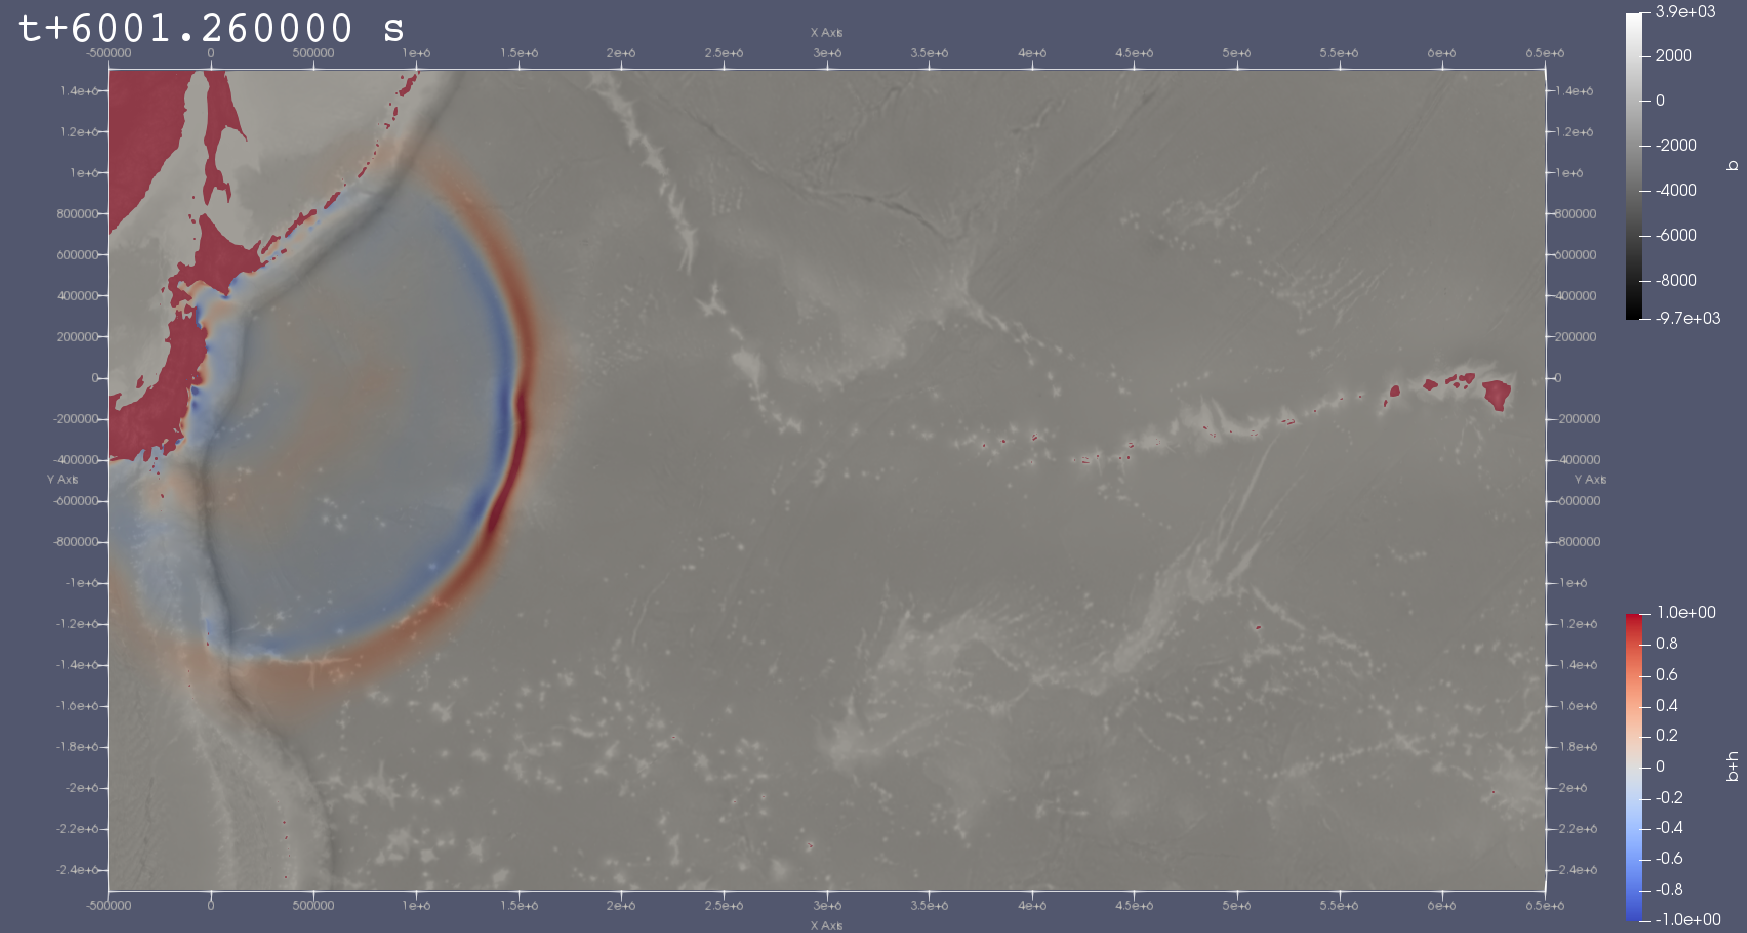
\includegraphics[clip,width=\linewidth]{img/tohoku_prod_sc_200.png}
						\caption*{Tuhoku scenario downscaled}
					}\only<4>{
						
\includegraphics[clip,width=\linewidth]{img/tuhoku_mixed.png}
						\caption*{Tuhoku HD / downscaled}
					}
		\end{figure}
	\end{multicols}
\end{frame}

\begin{frame}{Project}
	\centering
	Stay tuned for the project...
\end{frame}

\begin{frame}{Project}
	\textbf{Development of a graphical data analyzer}
	\begin{itemize}
		\item Standalone visualization of the SWE simulation output
		\item Analysis functionality
		\begin{itemize}
			\item Cell data extraction and visualization over time
			\item Cross-section visualization
			\item Coastal damage assessment (max. wave height and speed)
		\end{itemize}
		\item Data export
		\begin{itemize}
			\item Images
			\item Graphs (i.e. cross-sections)
			\item Video
		\end{itemize}
	\end{itemize}
\end{frame}

%--- GUI colors ---
\definecolor{guitoolbar}{HTML}{565656}
\definecolor{guidata}{HTML}{76323F}
\definecolor{guiexport}{HTML}{C09F80}

\begin{frame}{Project}
	\textbf{User Interface}
	\begin{multicols}{2}
		\begin{itemize}
			\item Interactive scenario map rendering
			\begin{itemize}
				\item Pan \& Zoom
				\item Multi-layer support
				\item Cursor as data probe
			\end{itemize}
			\item \textcolor{guitoolbar}{Toolbar}
			\item \textcolor{guidata}{Raw data display}
			\item \textcolor{guiexport}{Image export tools}
		\end{itemize}
		
	\columnbreak
		\centering
		\begin{figure}
			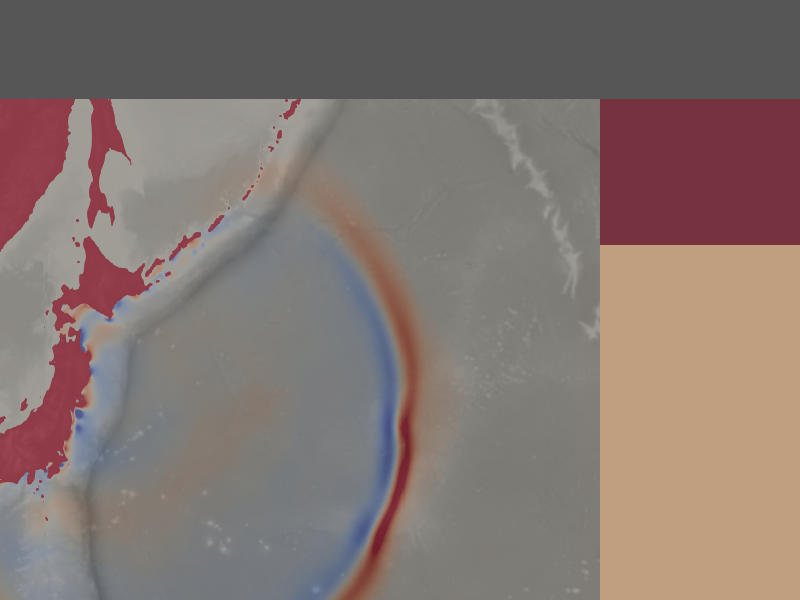
\includegraphics[clip,width=\linewidth]{img/GUI.png}
		\end{figure}	
	\end{multicols}
\end{frame}

\begin{frame}{Project}
	\textbf{Data analysis}
	\begin{itemize}
		\item Cell probe
		\item Arrival time calculator
		\item Cross-section analysis
	\end{itemize}
	
	\textbf{Export functionality}
	\begin{itemize}
		\item Images of the map
		\item Graphs (i.e. cross-sections)
		\item Videos
	\end{itemize}
\end{frame}

\begin{frame}{Project}
	\textbf{External libraries}\\\vspace{5pt}
	\begin{tabular}{ll}
		Framework & \textit{gtkmm} and \textit{glade}\\
		Renderer & \textit{openGL} pixelshader\\
		Image and video export & ffmpeg
	\end{tabular}
	\\\vspace{15pt}
	\textbf{Implementation}
	\begin{enumerate}
		\item Framework
		\item Height-map renderer
		\item Data analysis functionality
		\item Interactive GUI elements
		\item Zoom/pan of the map
		\item Image and video export
	\end{enumerate}
\end{frame}

\begin{frame}{}
	\begin{figure}
		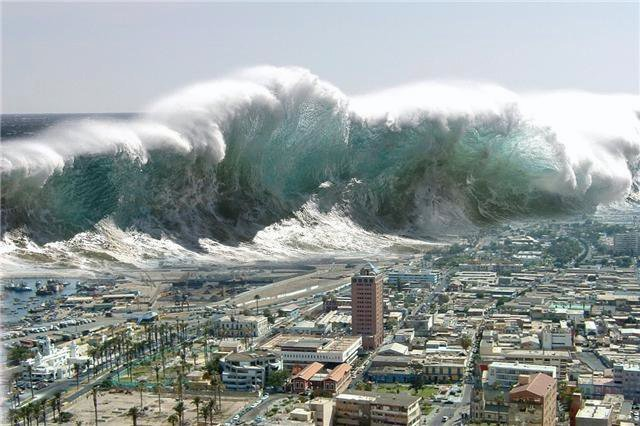
\includegraphics[clip, width=\imgfullscale\linewidth]{img/tsunami.jpg}
	\end{figure}
	\centering
	Thank you for your attention
	\\
	\vfill
	\flushleft
	{\fontsize{5}{5} \selectfont http://userscontent2.emaze.com/images/88c09d66-4283-49c0-9f80-9eb8fd05e30f/16101782-ea98-4b06-b114-4637be705926.jpg}
\end{frame}
	\end{document}